\documentclass{beamer}
%[aspectratio=169]   \usepackage[czech]{babel}
\usepackage{apo-lecture-en}
\usepackage{pdfpages}
\usepackage{pdfcomment}
\usepackage{listings}
\usepackage{array,multirow}

\subtitle{Lecture 05. Pipelined execution}
\author{Pavel Píša \phantom{xxxxxxx} Petr Štěpán \\ \small\texttt{pisa@fel.cvut.cz}\phantom{xxxx}\small\texttt{stepan@fel.cvut.cz}}
\begin{document}

\maketitle

\section{Pipelined execution}

\begin{frame}
\frametitle{The aim of today's lecture}

\begin{itemize}
 \item Suggest modifications to the processor from lecture 3 to use pipelining to make it faster
 \item Still consider the following instructions: \texttt{add}, \texttt{sub}, \texttt{and}, \texttt{or}, \texttt{slt}, \texttt{addi}, \texttt{lw}, \texttt{sw}, and \texttt{beq}
 \item Instruction coding also remains
\end{itemize}

\begin{table}
\footnotesize
\begin{tabular}{|m{0.4cm}|m{0.4cm}|m{1.0cm}|m{1.0cm}|m{0.4cm}|m{1.0cm}|m{1.0cm}|m{1.0cm}|m{0.4cm}|m{1.0cm}|}\hline
Typ & 31 & 30...25 & 24...21 & 20 & 19...15 & 14...12 & 11...8 & 7 & 6...0 \\ \hline
R & \multicolumn{2}{c|}{ fnct7 } & \multicolumn{2}{c|}{ rs2 } & rs1 & fnct3 &\multicolumn{2}{c|}{ rd } & opcode\\ \hline
I & \multicolumn{4}{c|}{ imm[11:0] } & rs1 & fnct3 &\multicolumn{2}{c|}{ rd } & opcode\\ \hline
S & \multicolumn{2}{c|}{ imm[11:5] } & \multicolumn{2}{c|}{ rs2 } & rs1 & fnct3 &\multicolumn{2}{c|}{ imm[4:0] } & opcode\\ \hline
B & imm [12] & imm [10:5]  & \multicolumn{2}{c|}{ rs2 } & rs1 & fnct3 & imm[4:1]& imm [11] & opcode\\ \hline
U & \multicolumn{6}{c|}{ imm[31:12] }  & \multicolumn{2}{c|}{ rd } & opcode\\ \hline
J & imm [20] & \multicolumn{2}{c|}{ imm[10:1] } & imm [11] & \multicolumn{2}{c|}{ imm[19:12] } & \multicolumn{2}{c|}{ rd } & opcode\\ \hline
\end{tabular}
\end{table}

\end{frame}

\begin{frame}
\frametitle{Single-cycle processor with memory (from lecture 3)}
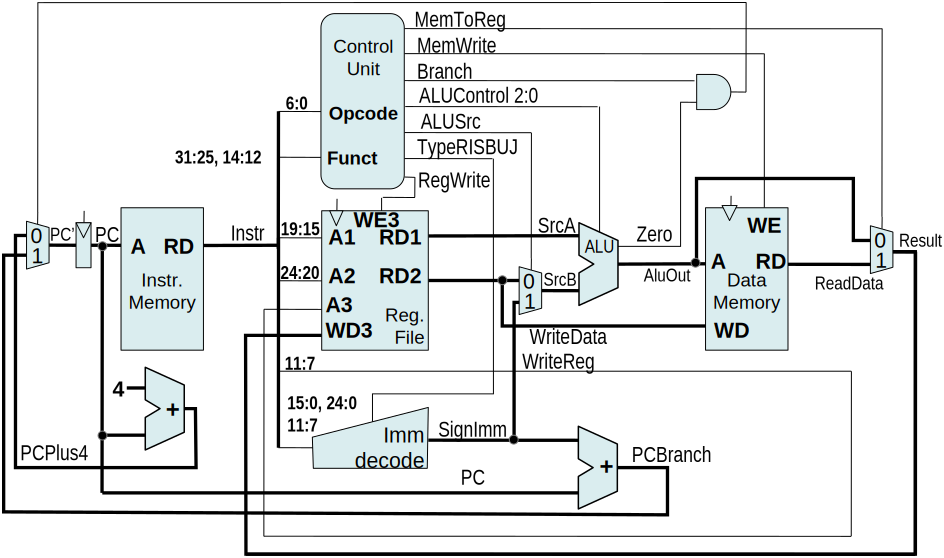
\includegraphics[width=0.95\textwidth]{single_cpu.pdf}
\end{frame}

\begin{frame}
\frametitle{The throughput of a single-cycle processor is limited}

\begin{itemize}
 \item Maximum instructions per second $IPS = IC / T = IPC_{avk} \cdot f_{clk}$
 \item Limited by the longest signal transit time from the remembered value to the input of the register (critical path)
 \item In our design, the constraints from the critical path of the \texttt{lw} instruction
\end{itemize}

\includegraphics[width=0.92\textwidth]{cpu-time.pdf}
\end{frame}

\begin{frame}
\frametitle{Critical path limiting throughput}

$f_{clk} = 1 / T_{C}$ where $T_{C}$ is the period of hours/time to process one cycle

\vskip 2 mm

$T_{C} = t_{PC} + t_{Mem} + t_{RFread} + t_{ALU} + t_{Mem} + t_{Mux} + t_{RFsetup}$

\vskip 2 mm

We consider the following delays and time requirements

\vskip 2 mm

\begin{tabular}{l c r}
$t_{PC}$ & = & $30$ ns \\
$t_{Mem}$ & = & $300$ ns \\
$t_{RFread}$ & = & $150$ ns \\
$t_{ALU}$ & = & $200$ ns \\
$t_{Mux}$ & = & $20$ ns \\
$t_{RFsetup}$ & = & $20$ ns \\
\end{tabular}

\vskip 2 mm

$T_{C} = 1020$\,ns $\rightarrow$ $f_{clk max} = 980$\,kHz

\vskip 2 mm

$IPS = IC / T = IPC_{avg} \cdot f_{clk}$

\vskip 2 mm

$IPS = 1 \cdots 980e3 = 980\,000$ instructions per second

\end{frame}

\begin{frame}
\frametitle{Split of instruction fetch and execution}

\begin{itemize}
 \item Fetching an instruction and reading it from memory ($2 \times t_{Mem}$) usually accounts for a significant part of the total cycle time
 \item It helps to reduce the cycle time if an instruction is already loaded in a previous cycle
\end{itemize}

\vskip 2 mm

{
\centering

\includegraphics[width=0.8\textwidth]{cpu_ifetch_exe.pdf}
}

\vskip 2 mm

\begin{enumerate}
 \item Instruction fetch and instruction counter increment $PC = PC + 4$
 \item Actual execution of the instruction only in the next loop
\end{enumerate}

\end{frame}

\begin{frame}
\frametitle{Processor modification for instruction prefetching}
\includegraphics[width=0.95\textwidth]{cpu_clock.pdf}
\begin{itemize}
 \item $\downarrow$ in the figure represents the clock input active on the rising edge of the clock signal
\end{itemize}

\end{frame}

\begin{frame}
\frametitle{Critical path in case of prefetching}

For the previously considered parameters

\vskip 2 mm

\begin{tabular}{l c r m{1 cm} l c r}
$t_{PC}$ & = & $30$ ns & & $t_{Mem}$ & = & $300$ ns \\
$t_{RFread}$ & = & $150$ ns  & & $t_{ALU}$ & = & $200$ ns \\
$t_{Mux}$ & = & $20$ ns  & & $t_{RFsetup}$ & = & $20$ ns \\
\end{tabular}

\vskip 2 mm

\begin{itemize}
 \item We consider $T_{C_{fetch}} = t_{PC} + t_{Mem}$ running in parallel with the execution of the instruction
 \item $T_{C_{exec}} = t_{RFread} + t_{ALU} + t_{Mem} + t_{Mux} + t_{RFsetup}$
\end{itemize}

after setting

\begin{itemize}
 \item Consider $T_{C_{fetch}} = 30 + 300 = 330$\,ns
 \item $T_{C_{exec}} = 150 + 200 + 300 + 20 + 20 = 690$\,ns
 \item $T_{C_{fetch}} < T_{C_{exec}}$ so $T_{C} = T_{C_{exec}} = 690$\,ns
 \item $\rightarrow f_{C} = 1.45$\,MHz $\rightarrow IPS = 1\,450\,000$
\end{itemize}

Without modifications, the delay of the jump instructions (\texttt{beq}) will occur, see later in the lecture

\end{frame}

\section{Five-stage pipeline}

\begin{frame}
\frametitle{Pipelined instruction execution}

We will consider splitting instruction execution into five stages.

\vskip 2 mm

{
\centering
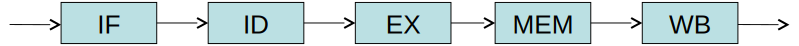
\includegraphics[width=0.9\textwidth]{cpu_pipe_stages.pdf}
}

\begin{enumerate}
 \item \textbf{IF} instruction fetch \textbf{Instruction Fetch} -- bringing \textbf{PC} to the memory address input, fetching the instruction and preparing $PC = PC + 4$ in parallel
 \item \textbf{ID} instruction decode \textbf{Instruction Decode} -- decode opcode, immediate operand and fetch registers according to \texttt{rs1} and \texttt{rs2} fields
 \item \textbf{EX} instruction execution \textbf{EXecution} -- execution of the requested function, passing register values and ALU constants
 \item \textbf{MEM} memory accesses \textbf{MEMory} -- if requested, memory writes (\textbf{sw}) or reads (\textbf{lw}) are performed at this stage
 \item \textbf{WB} register update \textbf{WriteBack} -- write the result to the register array for intermediate register instructions and memory
\end{enumerate}

\end{frame}

\begin{frame}
\frametitle{Overlapping sequential execution of instructions}
\includegraphics[width=0.9\textwidth]{cpu_pipe_inst_flow.pdf}

$\tau = max{\left\lbrace \tau_i \right\rbrace}^k_{i=1}$, where $\tau_i$ is the delay in each stage

It takes $n$ instructions to execute $k$ stages of chained processing
$$T_{k,n} = k \cdot \tau + (n - 1) \tau$$
Speedup
\hskip 7mm
$S_{k,n} = \frac{T_{1,n}}{T_{k,n}} = \frac{n k \tau}{k \tau + (n - 1) \tau}$
\hskip 7mm
$\lim_{n \rightarrow \infty} S_k = k$

\end{frame}

\begin{frame}
\frametitle{Single cycle processor (from lecture 3) -- datapath}
\includegraphics[width=0.95\textwidth]{cpu_nopipe.pdf}
\end{frame}

\begin{frame}
\frametitle{Stringed five-step design -- datapath}
\includegraphics[width=0.95\textwidth]{cpu_pipe.pdf}
\end{frame}

\begin{frame}
\frametitle{Stringed five-stage design including controller}
\includegraphics[width=0.95\textwidth]{cpu_ctrl_pipe.pdf}
\end{frame}

\section{Hazard emergence and resolution}

\begin{frame}
\frametitle{Data and control hazards and their treatment}
\includegraphics[width=0.95\textwidth]{hazard_kinds.pdf}
\end{frame}

\begin{frame}
\frametitle{Source of data hazards}
\includegraphics[width=0.95\textwidth]{hazard_data.pdf}

\vskip 2 mm

\begin{itemize}
 \item The register file is accessed from two stages (Decode, WriteBack) --
       writing is done in the first half of the loop, reading in the second half $\Rightarrow$ in the sub instruction to enter \textbf{s0} hazard is not created
 \item Read-After-Write (RAW) hazard occurs in instructions
       \textbf{and} and \textbf{or} when reading \textbf{s0} in steps 3 and 4
 \item How to avoid such hazard without degrading pipeline throughput?
\end{itemize}

\end{frame}


\begin{frame}
\frametitle{Data hazard in the "and" instruction tracked in the simulator}
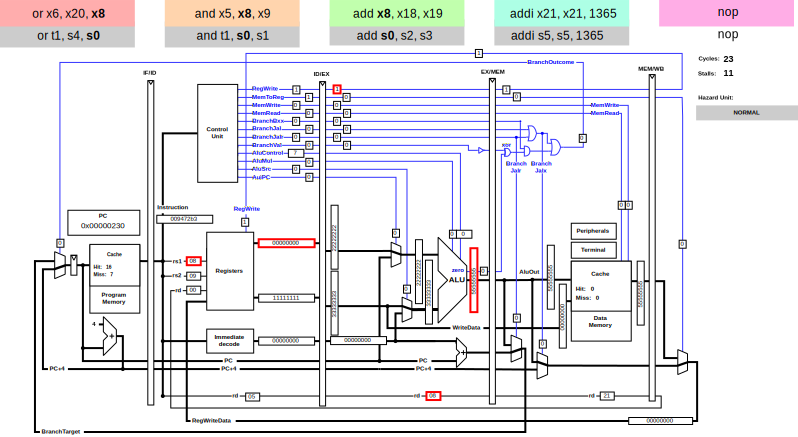
\includegraphics[width=0.95\textwidth]{hazard_qtrvsim.pdf}

{\tiny
QtRvSim \url{https://github.com/cvut/qtrvsim}
}

{\Tiny
\url{https://gitlab.fel.cvut.cz/b35apo/stud-support/-/blob/master/seminaries/qtrvsim/hazards-from-lecture/alu-hazards.S}
}

\end{frame}

\begin{frame}
\frametitle{Solving data hazard by stalling}
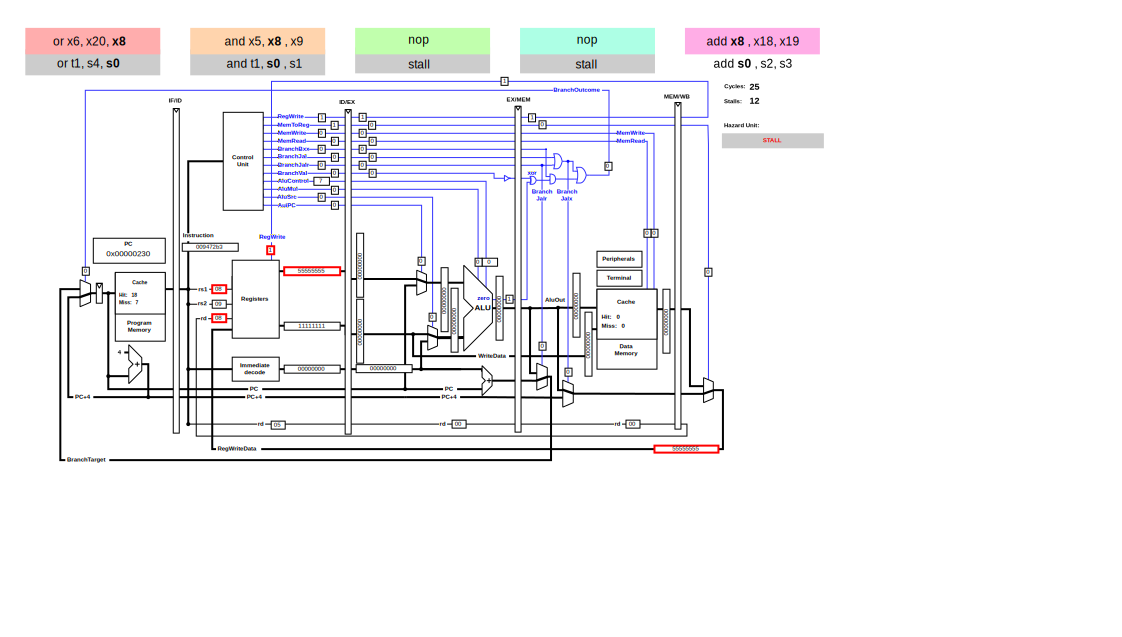
\includegraphics[width=0.95\textwidth]{hazard_stall_qtrvsim.pdf}

{\tiny
QtRvSim \url{https://github.com/cvut/qtrvsim}
}

{\Tiny
\url{https://gitlab.fel.cvut.cz/b35apo/stud-support/-/blob/master/seminaries/qtrvsim/hazards-from-lecture/alu-hazards.S}
}

\end{frame}


\begin{frame}
\frametitle{Data hazard resolution by forwarding}
\includegraphics[width=0.85\textwidth]{forward_data.pdf}

\begin{itemize}
 \item If the result is available (calculated) before the next instruction(s), which requires the result, is executed, the data hazard can be resolved by forwarding the value
 \item Data hazard occurs in the considered design if a source register
       (\textbf{rs1}, \textbf{rs2}) in the \textbf{EX} stage corresponds to the target register
       in \textbf{MEM} or \textbf{WB} (except X0/zero)
 \item The register numbers from the given stages are mapped to the Hazard Unit (HU)
\end{itemize}

\end{frame}

\begin{frame}
\frametitle{Recap of previous design and preparation for forwarding}
\includegraphics[width=0.95\textwidth]{noforward_data.pdf}

You need to know the previous \textbf{A1} (\textbf{rs1}) and \textbf{A2} (\textbf{rs2}) in \textbf{EX}.
The \textbf{RegWrite} signals from \textbf{MEM} and \textbf{WB} must also be monitored to confirm,
that the register specified by \textbf{WriteReg} in \textbf{MEM} and \textbf{WB} is indeed being written.

\end{frame}

\begin{frame}
\frametitle{Processor design with MEM and WB to EX forwarding}
\includegraphics[width=0.95\textwidth]{forward_hazard.pdf}
\end{frame}

\begin{frame}
\frametitle{QtRvSim -- data hazards resolved by forwarding}
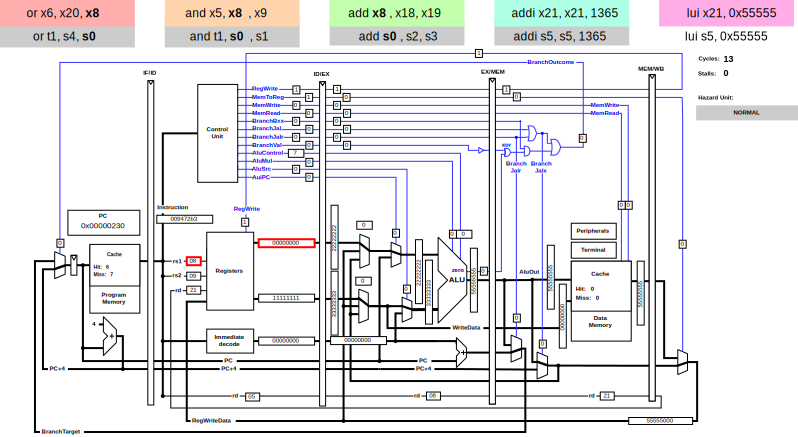
\includegraphics[width=0.95\textwidth]{hazard_forwarding.pdf}

{\tiny
QtRvSim \url{https://github.com/cvut/qtrvsim}
}

{\Tiny
\url{https://gitlab.fel.cvut.cz/b35apo/stud-support/-/blob/master/seminaries/qtrvsim/hazards-from-lecture/alu-hazards.S}
}

\end{frame}

\begin{frame}
\frametitle{QtRvSim -- forwarding the "and" instruction input from MEM}
\includegraphics[width=0.95\textwidth]{hazard_forwarding2.pdf}

{\tiny
QtRvSim \url{https://github.com/cvut/qtrvsim}
}

{\Tiny
\url{https://gitlab.fel.cvut.cz/b35apo/stud-support/-/blob/master/seminaries/qtrvsim/hazards-from-lecture/alu-hazards.S}
}

\end{frame}

\begin{frame}
\frametitle{QtRvSim -- forwarding the input of the "or" instruction from WB}
\includegraphics[width=0.95\textwidth]{hazard_forwarding3.pdf}

{\tiny
QtRvSim \url{https://github.com/cvut/qtrvsim}
}

{\Tiny
\url{https://gitlab.fel.cvut.cz/b35apo/stud-support/-/blob/master/seminaries/qtrvsim/hazards-from-lecture/alu-hazards.S}
}

\end{frame}

\begin{frame}
\frametitle{Persisting problem in the "lw" instruction -- solved by stalling}
\includegraphics[width=0.85\textwidth]{pipeline_stall.pdf}

\begin{itemize}
 \item If the following instruction requires data before it is available in the processor, it is necessary to
       suspend the pipeline (\textbf{stall}) and stall/\textbf{nop} is inserted into the continuation pipeline
       states
 \item Stalling solves hazards but degrades throughput
 \item Stages preceding the stage affected by the hazard are suspended until all others are
       results required by other instructions are available -- the results are then forwarded to all locations where
       the required
\end{itemize}

\end{frame}

\begin{frame}
\frametitle{Data hazard resolution by stalling}
\includegraphics[width=0.85\textwidth]{pipeline_stall2.pdf}

\begin{itemize}
 \item Stalling is implemented by holding the contents of the interstage registers
       (by gating their clock or recording signals)
 \item Results from stages with missing data are not used, signals
       for writing to memory and registers and other control signals  are reset
 \item Both are achieved by adding control signals for delay or
       zeroing of intermediate registers
\end{itemize}

\end{frame}

\begin{frame}
\frametitle{Solve remaining data hazards by stalling}
\includegraphics[width=0.95\textwidth]{cpu_fwd_stall.pdf}
\end{frame}

\begin{frame}
\frametitle{QtRvSim -- data hazard in "lw" solved by stalling}
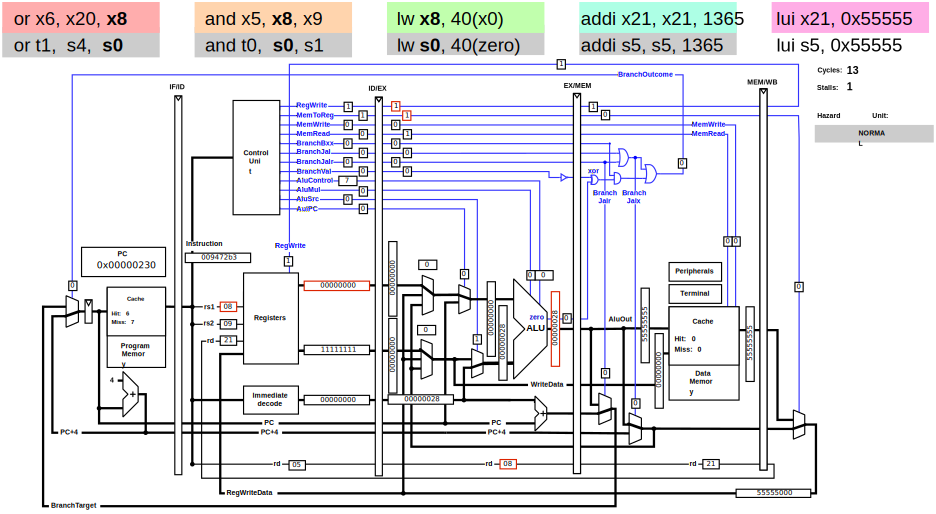
\includegraphics[width=0.95\textwidth]{hazard_stall_qtrvsim2.pdf}
{\tiny
QtRvSim \url{https://github.com/cvut/qtrvsim}
}

{\Tiny
\url{https://gitlab.fel.cvut.cz/b35apo/stud-support/-/blob/master/seminaries/qtrvsim/hazards-from-lecture/lw-hazards.S}
}

\end{frame}

\begin{frame}
\frametitle{QtRvSim -- data hazard in "lw" solved by stalling}
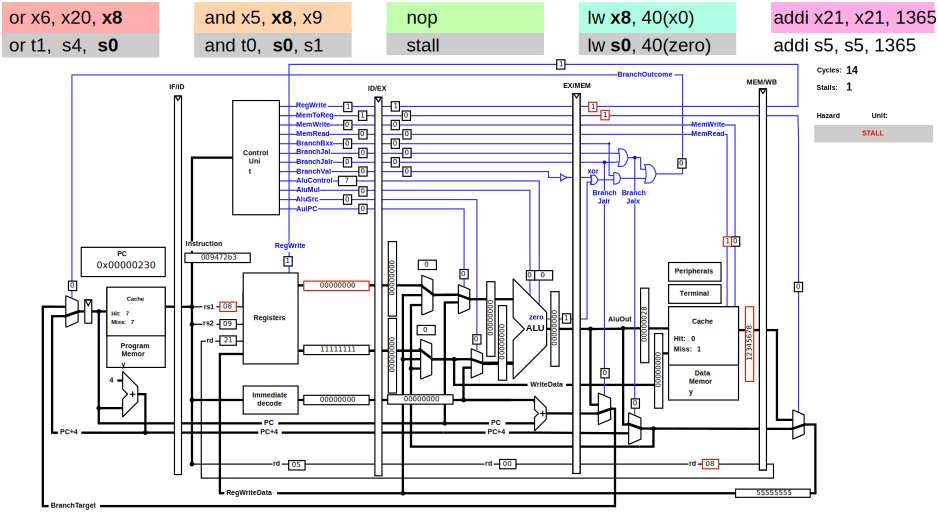
\includegraphics[width=0.95\textwidth]{hazard_stall_qtrvsim3.pdf}

{\tiny
QtRvSim \url{https://github.com/cvut/qtrvsim}
}

{\Tiny
\url{https://gitlab.fel.cvut.cz/b35apo/stud-support/-/blob/master/seminaries/qtrvsim/hazards-from-lecture/lw-hazards.S}
}

\end{frame}

\begin{frame}
\frametitle{QtRvSim -- data hazard in "lw" solved by stalling}
\includegraphics[width=0.95\textwidth]{hazard_stall_qtrvsim4.pdf}

{\tiny
QtRvSim \url{https://github.com/cvut/qtrvsim}
}

{\Tiny
\url{https://gitlab.fel.cvut.cz/b35apo/stud-support/-/blob/master/seminaries/qtrvsim/hazards-from-lecture/lw-hazards.S}
}

\end{frame}

\section{Control hazards}

\begin{frame}
\frametitle{Control hazards (branch and jump instructions)}
\includegraphics[width=0.85\textwidth]{hazard_ctrl.pdf}

\begin{itemize}
 \item The result is not known until the fourth cycle, then it is loaded to the PC
       and so the first instruction at the jump target address may not be loaded until cycle five.
 \item Jumps in this way represent a major limitation on the time usage of the execution units in the pipeline
\end{itemize}

\end{frame}

\begin{frame}
\frametitle{Alternative, move jump decision making earlier}
\includegraphics[width=0.85\textwidth]{hazard_ctrl2.pdf}

\begin{itemize}
 \item A structural hazard is created, \textbf{ALU} is needed in both \textbf{EX} and \textbf{ID}.
 \item Structural hazards can be solved by duplicating elements. A complete adder, subtractor or comparison
       takes a long time, a solution may be to restrict the jump conditions to match/mismatch only (just xor
       between operands and nor over bits)
\end{itemize}

\end{frame}

\begin{frame}
\frametitle{Jump execution to ID -- MIPS architecture}
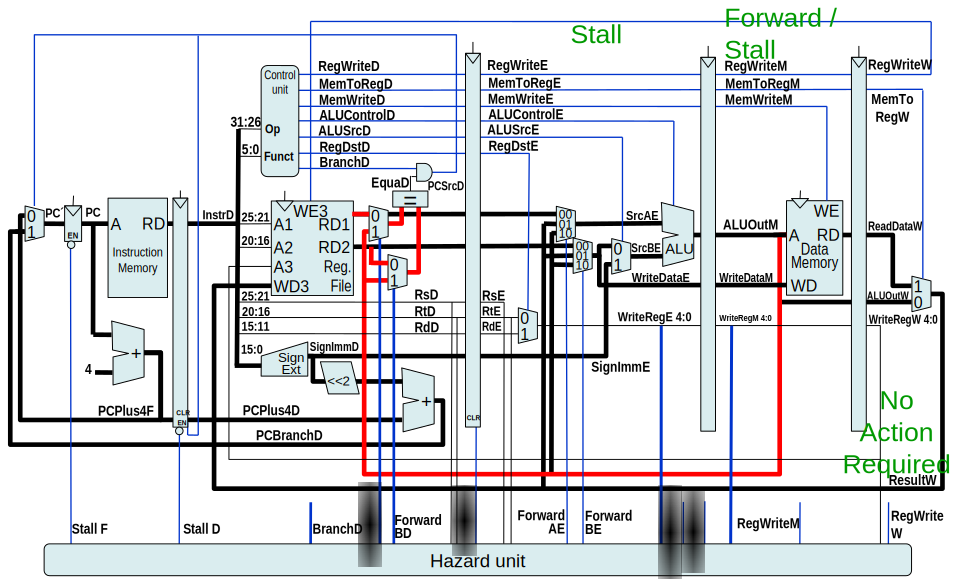
\includegraphics[width=0.90\textwidth]{hazard_ctrl_mips2.pdf}
\end{frame}

\begin{frame}
\frametitle{Hazard resolution on comparator inputs -- MIPS}
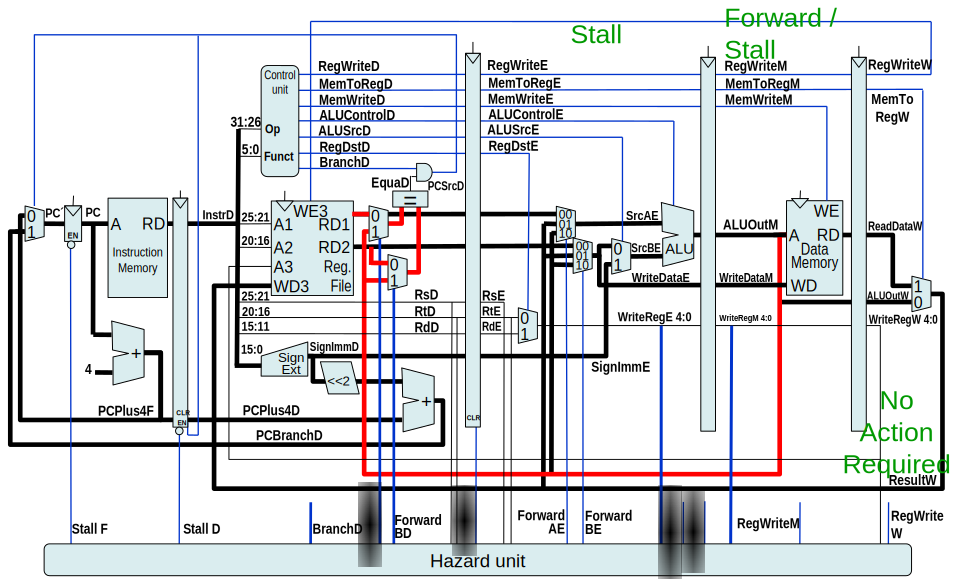
\includegraphics[width=0.90\textwidth]{hazard_ctrl_mips2.pdf}
\end{frame}

\begin{frame}
\frametitle{Jump prediction and speculative instruction execution (next time)}
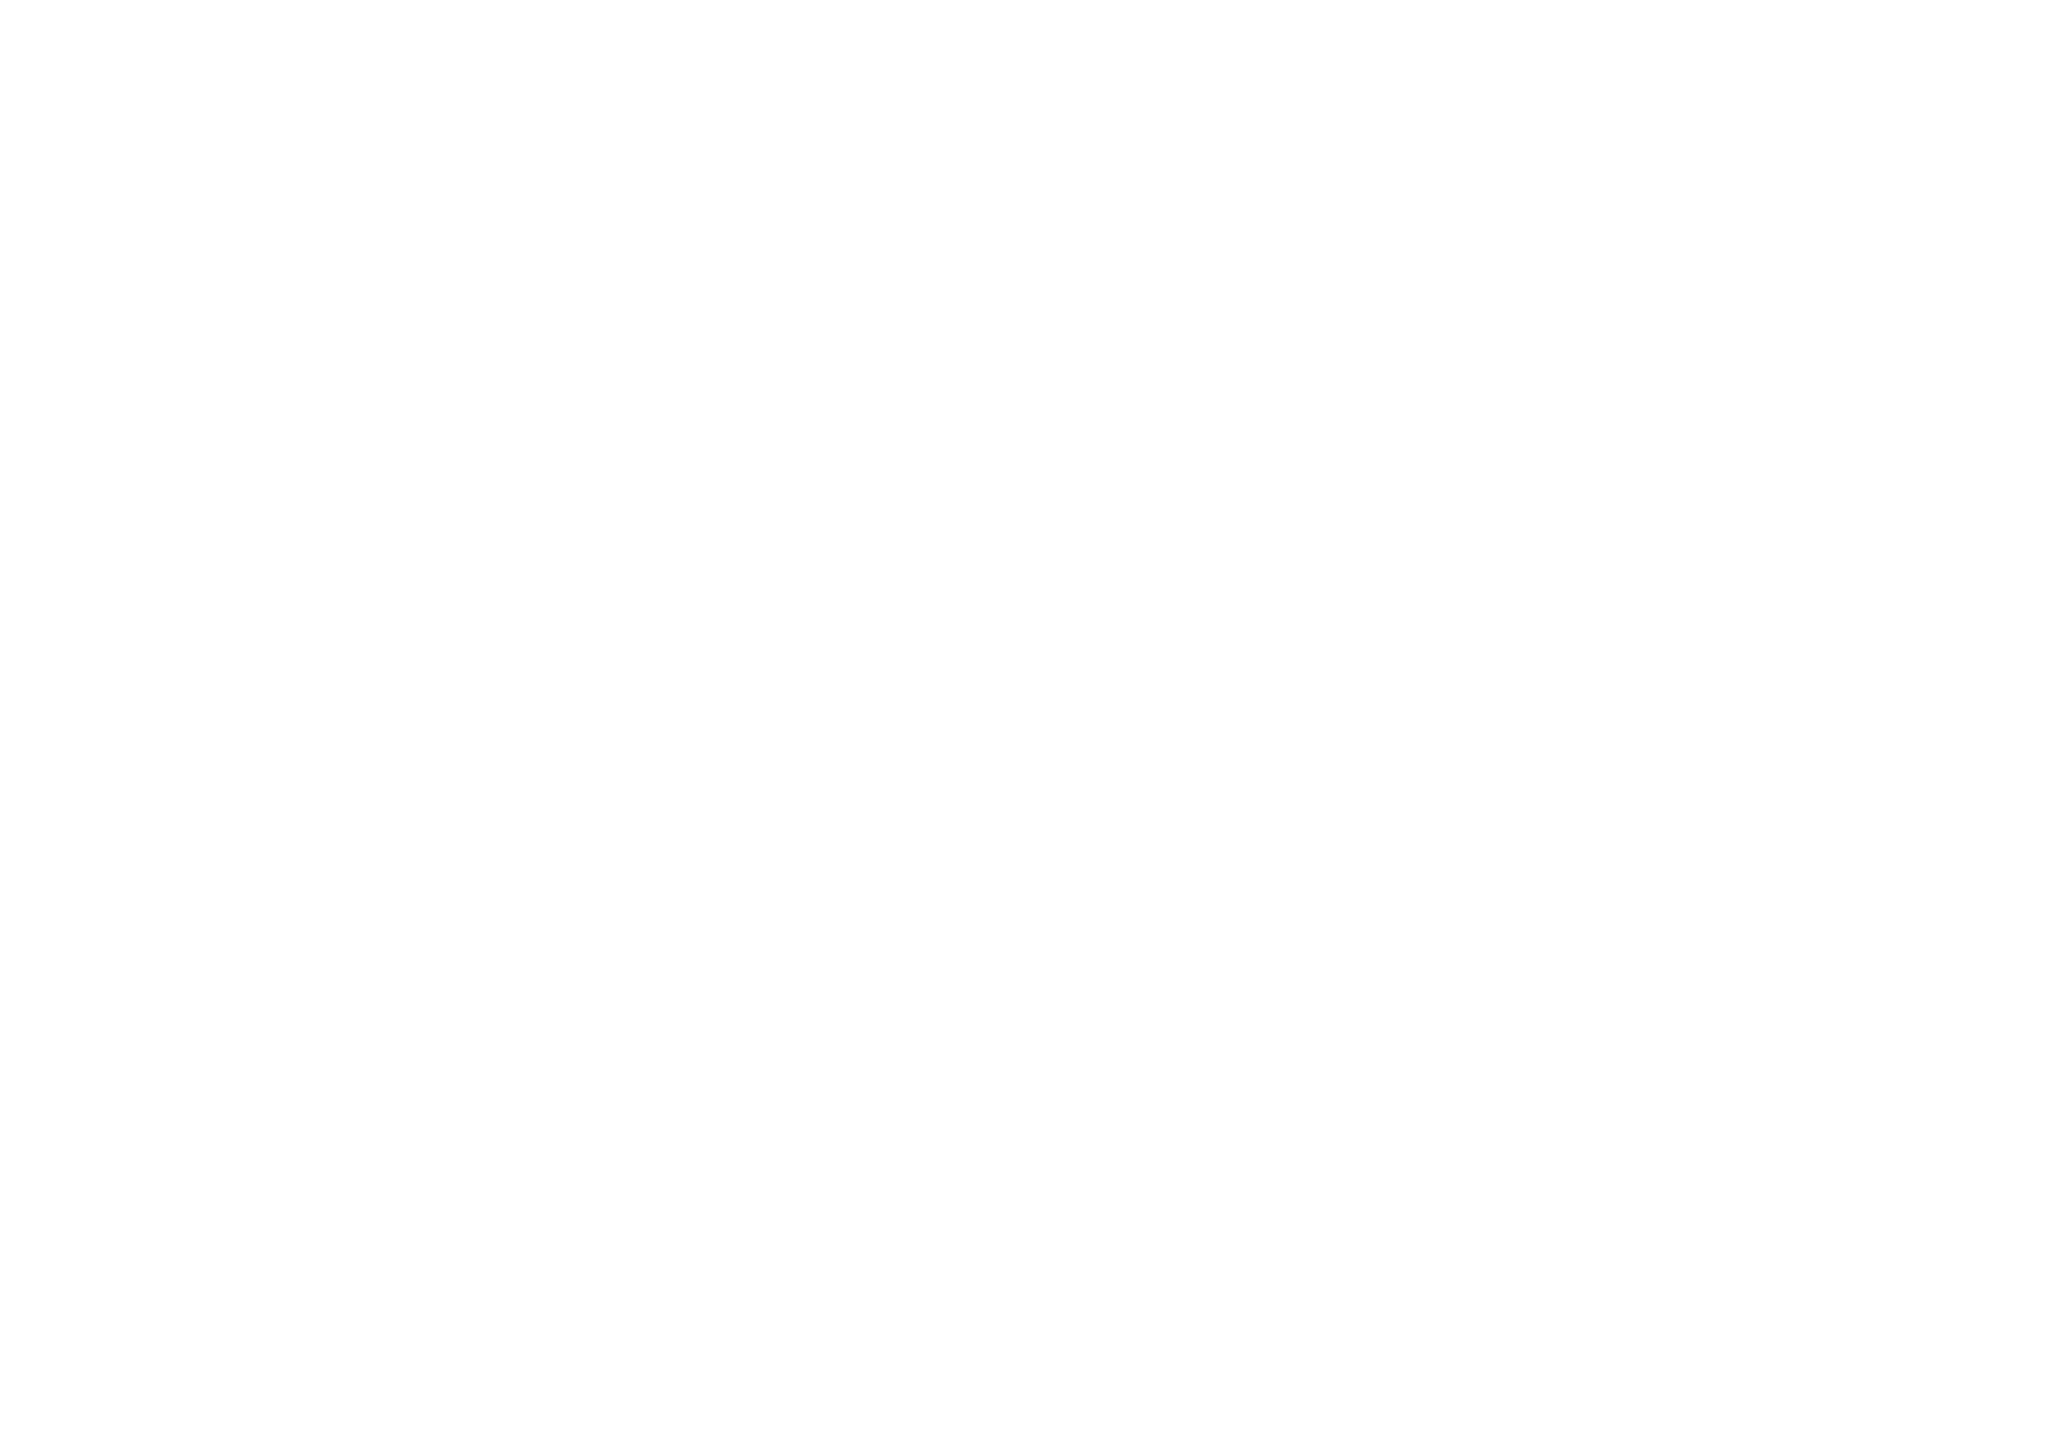
\includegraphics[width=0.90\textwidth]{cpu_branch_pred.pdf}
\end{frame}

\begin{frame}
\frametitle{Result of pipelined processor design -- RISC-V}
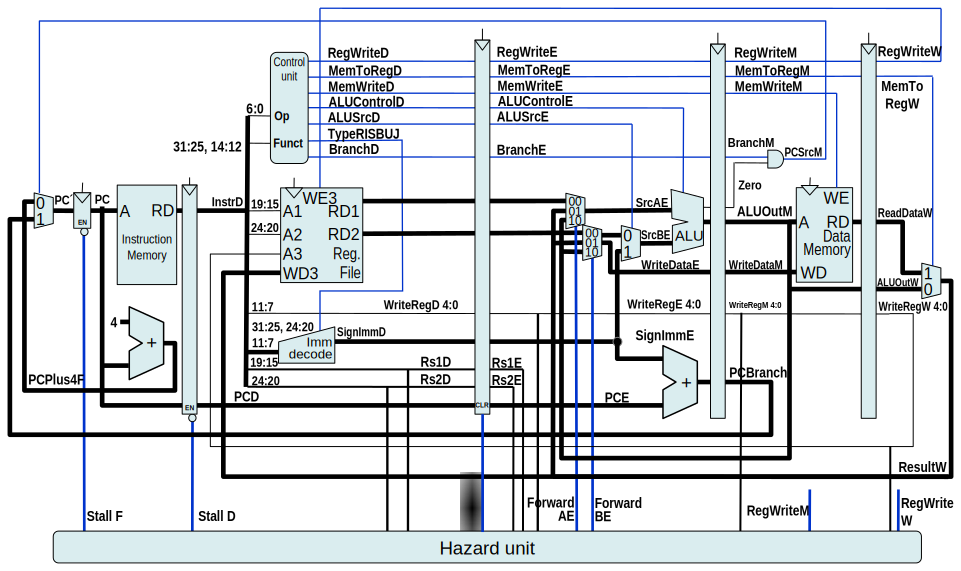
\includegraphics[width=0.95\textwidth]{cpu_final_design.pdf}
\end{frame}

\begin{frame}
\frametitle{Bandwidth of the proposed pipelined processor}

\begin{itemize}
 \item What will be the maximum achievable frequency of the processor?
 \item Which stage is the slowest?
 \item The minimum allowable cycle period is given by the slowest stage
 \item In our case, we are dealing with memory \\
       $T_C = 300$\,ns $\rightarrow$ $f_{clk\,max} = 3\,333$\,kHz \\
       if we don't consider extra cycles to fill the pipeline (no pauses
       and emptying during jumps, for example) then for an ideal $IPC = 1$ \\
       $IPS = 1 \cdot 3\,333e3 = 3\,333\,000$ instructions per second
 \item The introduction of five-stage chained processing has led to an increase in
       throughput of $3\,333\,000 / 980\,000 = 3.4 \times$ assuming $IPC = 1$
\end{itemize}

\end{frame}

\section{Processor with memory}

\begin{frame}
\frametitle{How does the design correspond to a real processor with memory attached (for simplicity we don't consider the pipeline)}
\includegraphics[width=0.95\textwidth]{cpu_design.pdf}
\end{frame}

\begin{frame}
\frametitle{Memory will no longer be considered on chip}
\includegraphics[width=0.95\textwidth]{cpu_design2.pdf}
\end{frame}

\begin{frame}
\frametitle{We're going back to the original CPU, memory split}
\includegraphics[width=0.85\textwidth]{cpu_design3.pdf}
\end{frame}

\begin{frame}
\frametitle{Which instruction fails on a link break}
\includegraphics[width=0.95\textwidth]{cpu_final_design_bonus.pdf}

\textbf{A)} add \hfill \textbf{B)} addi \hfill \textbf{C)} beq \hfill \textbf{D)} or \hfill ?
\end{frame}

\section{Real design considerations and constraints (for A grade adepts)}

\begin{frame}
\frametitle{Requirements for Pipeline Timing}
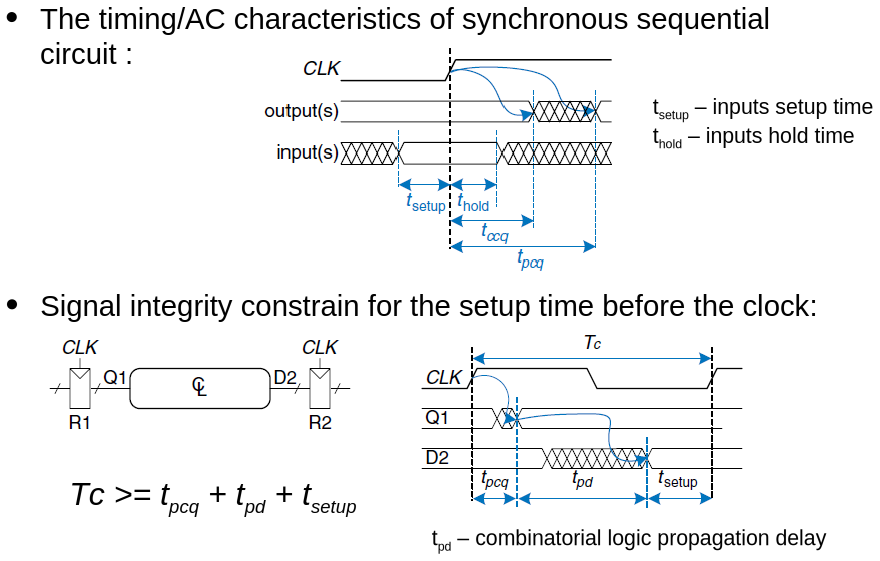
\includegraphics[width=0.95\textwidth]{pipeline_timing1.pdf}
\end{frame}

\begin{frame}
\frametitle{Requirements for Pipeline Timing}
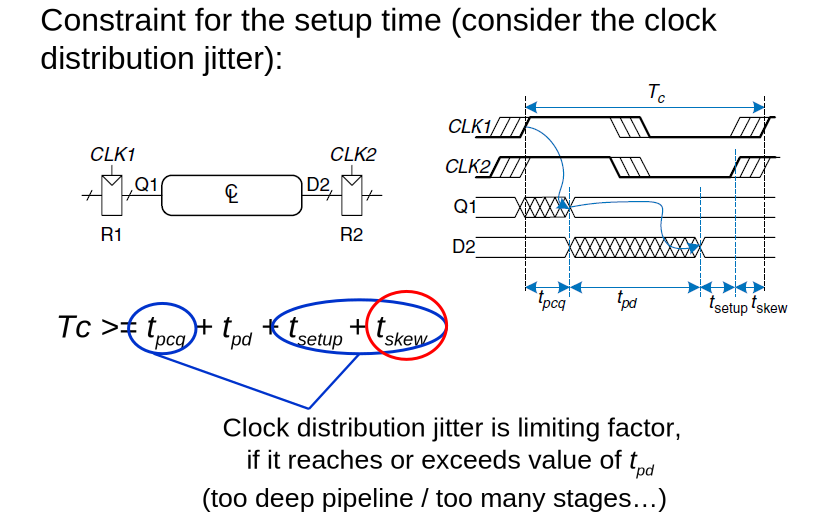
\includegraphics[width=0.95\textwidth]{pipeline_timing2.pdf}
\end{frame}

\begin{frame}
\frametitle{Clock Distribution Network Skew}
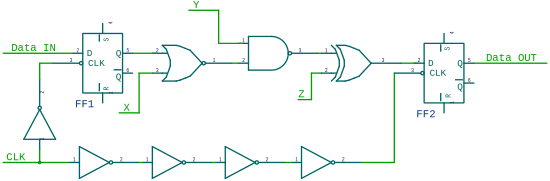
\includegraphics[width=0.9\textwidth]{clock_distribution_skew.pdf}

\begin{itemize}
 \item \textbf{Positive Clock Skew} -- clock arrives at the capturing sequential later than it arrives at the launching sequential
 \item \textbf{Negative Clock Skew} -- clock arrives at the launching sequential later than it arrives at the capturing sequential
 \item \textbf{Local Clock Skew} -- skew between any two sequentials with a valid timing path between them.
 \item \textbf{Global Clock Skew} -- clock skew between any two sequentials in the design regardless of whether a timing paths exists between them
\end{itemize}

\end{frame}

\begin{frame}
\frametitle{Clock Distribution Network -- H-tree}

{
\centering
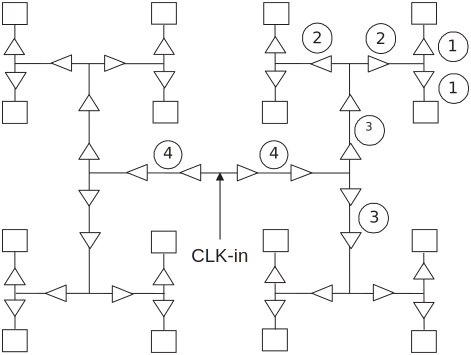
\includegraphics[width=0.6\textwidth]{clock_distribution_h_tree.pdf}
}

\vskip 2mm

source: Tawfik, S., Kursun, V.: Clock Distribution Networks with Gradual Signal Transition Time Relaxation for Reduced Power Consumption.

\end{frame}

\begin{frame}
\frametitle{Pipeline Stages Balancing}
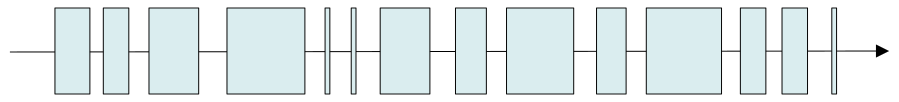
\includegraphics[width=0.85\textwidth]{pipeline_balancing.pdf}

(applies to tree based adder, multiplier, (unrolled) iterative divider..)

\begin{itemize}
 \item \textbf{Balancing}: the goal is to divide the processing into N stages in such a way, that stage propagation delays are roughly the same...
 \item The number of stages reflects preference of \underline{performance} (\underline{throughput}) versus latency.
\end{itemize}

\end{frame}

\begin{frame}
\frametitle{Superpipeline and Beyond}

\begin{itemize}
 \item Not well balanced 5-stage pipeline:
\end{itemize}

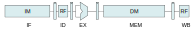
\includegraphics[width=0.85\textwidth]{pipeline_balancing2.pdf}

\begin{itemize}
 \item Deeper pipeline is result of decomposing stages into more stages
\end{itemize}

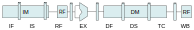
\includegraphics[width=0.85\textwidth]{pipeline_balancing3.pdf}

\begin{itemize}
 \item It allows CPU to work at higher frequencies but introduces many problems as well...
 \item Complex forwarding, more pipeline stalls, hazards need to be solved by complex logic
\end{itemize}

\end{frame}

\begin{frame}
\frametitle{Superpipeline and Beyond}

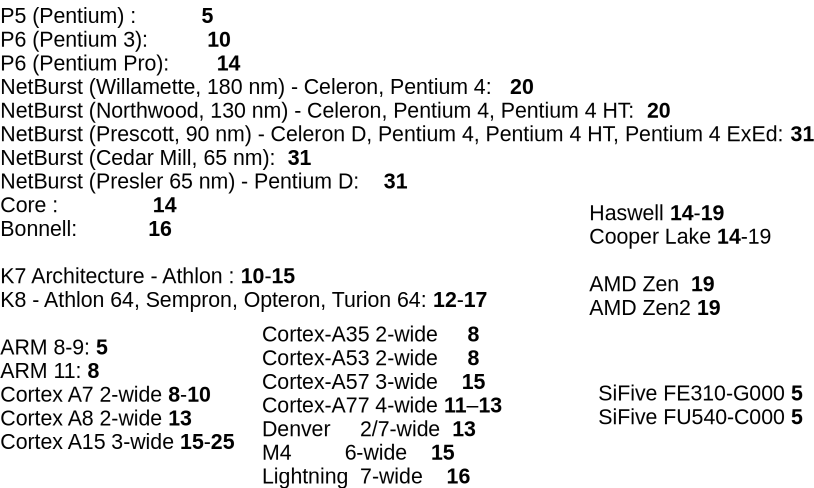
\includegraphics[width=0.95\textwidth]{pipeline_today_depths.pdf}

The Optimum Pipeline Depth for a Microprocessor: {\tiny \url{http://citeseerx.ist.psu.edu/viewdoc/download?doi=10.1.1.93.4333\&rep=rep1\&type=pdf}}

\end{frame}

\end{document}

